\documentclass[12pt]{article}
\usepackage{natbib}
\bibliographystyle{aasjournal}
\usepackage{latexsym}
\usepackage{graphicx}
\usepackage{epsfig}
\usepackage{amssymb}
\usepackage{amsmath}
\usepackage{epstopdf}

\usepackage{pb-diagram}

\parindent = 0.0 in
\parskip = 0.15 in

\newcommand\Beq{\begin{align}} 
\newcommand\Eeq{\end{align}}

\newcommand\Bfig{\begin{figure}} 
\newcommand\Efig{\end{figure}}

\newcommand\Ra{\mathrm{Ra}}
\newcommand\Pran{\mathrm{Pr}}
\newcommand\Rac{\mathrm{Ra}_{\mathrm{c}}}
\newcommand\Ek{\mathrm{Ek}}
\newcommand\Ro{\mathrm{Ro}}
\newcommand\Nu{\mathrm{Nu}}
\newcommand\Sc{\mathrm{Sc}}

\newcommand\eps{\varepsilon}
\renewcommand\L {\mathcal{L}}

\newcommand{\n}{\\ \nonumber \\ }
\newcommand{\nn}{\nonumber}
\newcommand{\nnn}{\\ \nonumber \\ \nonumber}

\newcommand\ie{\textit{i.e.},~}
\newcommand\eg{\textit{e.g.},~}
\newcommand{\omicron}{o}

\newcommand{\angles}[1]{\langle #1 \rangle}
\newcommand{\pd}[1]{\partial_{#1}}
\renewcommand{\vec}[1]{\boldsymbol{#1}}
\newcommand{\M}[1]{\mathbf{#1}}
\renewcommand{\dot}{\vec{\cdot}}
\newcommand{\grad}{\vec{\nabla}}
\newcommand{\cross}{\vec{\times}}
\newcommand{\laplacian}{\nabla^2}
\renewcommand{\bar}[1]{\overline{#1}}

\newcommand{\Fbot}{\ensuremath{F_{\rm{bot}}}}
\newcommand{\Ftot}{\ensuremath{F_{\rm{tot}}}}
\newcommand{\Frad}{\ensuremath{F_{\rm{rad}}}}
\newcommand{\Fconv}{\ensuremath{F_{\rm{conv}}}}
\newcommand{\Fcz}{\ensuremath{F_{\rm{cz}}}}
\newcommand{\mP}{\ensuremath{\mathcal{P}}}
\newcommand{\mB}{\ensuremath{\mathcal{B}}}


\newcommand{\sump}[2]{\sideset{}{'}\sum_{{#1}=0}^{#2}}

\newcommand{\eq}[1]{eq.~(\ref{#1})}
\newcommand{\eqs}[2]{eqs.~(\ref{#1})~\&~(\ref{#2})}
\newcommand{\eqss}[2]{eqs.~(\ref{#1})--(\ref{#2})}

\newcommand{\Eq}[1]{Eq.~(\ref{#1})}
\newcommand{\Eqs}[2]{Eqs.~(\ref{#1})~\&~(\ref{#2})}
\newcommand{\Eqss}[2]{Eqs.~(\ref{#1})--(\ref{#2})}

\newcommand{\fig}[1]{Fig.~(\ref{#1})}
\newcommand{\figs}[2]{Figs.~(\ref{#1})~\&~(\ref{#2})}

\newcommand{\tbl}[1]{Table~(#1)}

\newcommand{\aap}{A\&A}

\begin{document}

\section{Integral constraint}
Following arguments we've made a bunch of times, the time-stationary full convection zone (CZ and PZ) is bound by an integral constraint,
\begin{equation}
\int \bar{\mB}\,dz = \int \bar{\Phi}\,dz,
\end{equation}
where $\bar{\mB} \equiv \bar{\Fconv}$ is the buoyant KE generation rate and $\bar{\Phi} \equiv \mathcal{R}^{-1}\bar{|\vec{\omega}|^2}$ is the viscous dissipation rate.
We have generally found it instructive to break up the integrals above into CZ and PZ portions,
\begin{equation}
\int_{\rm{CZ}} \bar{\mB}\,dz = \int_{\rm{CZ}} \bar{\Phi}\,dz + \int_{\rm{PZ}} \bar{\Phi}\,dz + \int_{\rm{PZ}} (-\bar{\mB})\,dz,
\end{equation}
where the LHS represents the total work done by buoyancy in the convection zone, and the RHS represents the viscous and (negative) PZ buoyancy work that cancels that work.
We have typically moved on to divide this equation by the LHS and define the parameter,
\begin{equation}
f \equiv \frac{\int_{\rm{CZ}}\bar{\Phi}\,dz}{\int_{\rm{CZ}}\bar{\mB}\,dz},
\label{eqn:f_defn}
\end{equation}
and we have assumed that $f$ is a constant.
Unfortunately this is not in general true in our measurements, but it could be true in the infinite Reynolds number limit.

\section{Breaking out boundary layer contributions}
Further breaking apart the CZ integral into a bulk and BL contribution, the definition of Eqn.~\ref{eqn:f_defn} becomes
\begin{equation}
f \equiv 
\frac{\int_{\rm{bulk}}\bar{\Phi}\,dz}{\int_{\rm{CZ}}\bar{\mB}\,dz}
+
\frac{\int_{\rm{BL}}\bar{\Phi}\,dz}{\int_{\rm{CZ}}\bar{\mB}\,dz}.
\label{eqn:f_split}
\end{equation}
For simplicity, we will assume that $\bar{\Phi}$ is a constant value $\Phi_{\rm{CZ}}$ in the bulk of the convection zone.
This is a decent assumption which describes the simulations fairly well (but is not perfect).
We will then define
\begin{equation}
f_{\infty} \equiv \frac{\Phi_{\rm{CZ}} L_{\rm{CZ}}}{\int_{\rm{CZ}}\bar{\mB}\,dz},
\end{equation}
where here $L_{\rm{CZ}}$ is the depth of the full CZ from the bottom boundary to the upper Schwarzschild boundary (it's the range over with the $\int_{\rm{CZ}}$ integral is taken).
With this we can rewrite Eqn.~\ref{eqn:f_split},
\begin{equation}
f \approx f_{\infty} \frac{L_{\rm{bulk}}}{L_{\rm{CZ}}} + 
\frac{\int_{\rm{BL}}\bar{\Phi}\,dz}{\int_{\rm{CZ}}\bar{\mB}\,dz},
\label{eqn:f_approx}
\end{equation}
where $L_{\rm{bulk}} = L_{\rm{CZ}} - \delta_{\nu}$ is the depth of the bulk integral and $\delta_{\nu}$ is the viscous boundary layer depth.
To say more we need to talk about a specific type of boundary condition.

In general, in Rayleigh B\'{e}nard convection, we expect the viscous boundary layers to be the same size scale $\delta_{\nu} \sim \delta_{T}$ (where $\delta_T$ is the thermal boundary layer).
Furthermore, in RBC, the Nusselt number Nu $\sim \delta_T^{-1}$ and since essentially all RBC simulations are boundary controlled, $\rm{Nu} \propto \rm{Ra}^{1/3} \propto \rm{Re}^{2/3}$.
So we can generally expect boundary layers to scale like $\delta_{\nu} \propto \rm{Re}^{-2/3} \sim \mathcal{R}^{-2/3}$.
In our problem we have removed the bottom thermal boundary using our internal heating setup, so we can't really take the RBC intuition too much further and can't use it to bound $f$, for example.

\subsection{Stress-free boundaries}
In our simulations with stress-free boundaries, we see the dissipation decrease from its bulk value $\Phi_{\rm{CZ}}$ to a much lower value, close to zero, in the boundary layer.
As a zeroth order model, we can say $\int_{\rm{BL}}\bar{\Phi}\,dz \approx 0$, so Eqn.~\ref{eqn:f_approx} simply becomes the bulk portion,
\begin{equation}
f \approx f_{\infty}\left(1 - \frac{\delta_\nu}{L_{\rm{CZ}}}\right)
\sim
f_{\infty}\left(1 - \mathcal{R}^{-2/3}\right),
\label{eqn:stressfree_f}
\end{equation}
and we expect $f$ to converge to $f_{\infty}$ in the infinite Reynolds number limit.

\subsection{No-slip boundaries}
Here things are a bit more complicated.
Now the boundary layer is the location where dissipation peaks, because $\vec{u}$ must go from its bulk value $u_{\rm{rms}}$ to 0 at the boundary.
So we can estimate that the vorticity has a value $\omega \sim u_{\rm{rms}}/\delta_{\nu}$.
Thus the boundary layer dissipation is $\bar{\Phi_{\rm{BL}}} \approx \mathcal{R}^{-1} u_{\rm{rms}}^2/\delta_{\nu}^{2}$
Integrating this (constant) value over the boundary layer, we find
\begin{equation}
f \approx f_{\infty}\left(1 - \frac{\delta_\nu}{L_{\rm{CZ}}}\right) + \frac{C_0}{\mathcal{R}\delta_{\nu}}
\sim
f_{\infty}\left(1 - \mathcal{R}^{-2/3}\right) + C \mathcal{R}^{-1/3},
\end{equation}
where $C_0$ and $C$ are the sins of all of the constants I've been too lazy to carry along.
Anyways we see that in the infinite $\mathcal{R}$ limit, we get the same result $f_{\infty}$, but we have to go to higher $\mathcal{R}$ to get there.

\section{Dissipation in the penetration zone}
This remains a thorn in our side. 
I previously modeled this as linear but perhaps its best to model this as
\begin{equation}
\frac{\int_{\rm{PZ}}\bar{\Phi}\,dz}{\int_{\rm{CZ}}\bar{\mB}\,dz} \approx f\frac{\delta_p}{L_s}\xi,
\label{eqn:xi_defn}
\end{equation}
where $f$ is the same $f$ as above, $\delta_p$ is the penetration zone depth, $L_s$ is the schwarzshild-defined depth of the convection zone, and $\xi$ is a geometric factor that describes the shape of the dissipation in the PZ.
We can model the dissipation as a polynominally decreasing function,
\begin{equation}
\Phi_{\rm{PZ}} = \Phi_{\rm{CZ}}(1 - \tilde{z}^{n}),\qquad
\rm{with}\qquad
\tilde{z} = \frac{z - L_s}{\delta_p},
\end{equation}
where $\tilde{z}$ is a modified coordinate that is zero at the base of the PZ and 1 at the top of the PZ.
If we integrate,
\begin{equation}
\int_{0}^{1} \Phi_{\rm{CZ}}(1 - \tilde{z}^{n}) = \frac{n}{n+1}\Phi_{\rm{CZ}}.
\end{equation}
So we see that if $\Phi$ decreases linearly in the PZ ($n = 1$) then $\xi = 1/2$.
If $\Phi$ decreases quadratically then $\xi = 2/3$, and so on.
(This is not meant to be a perfect description, but we can measure $\xi$ in simulations and its value, combined with $n$ can give us a decent description).

\section{How does this look in the data?}
See Figs.~\ref{fig:profiles} and \ref{fig:f_and_xi}.
\begin{figure}[ht!]
\centering
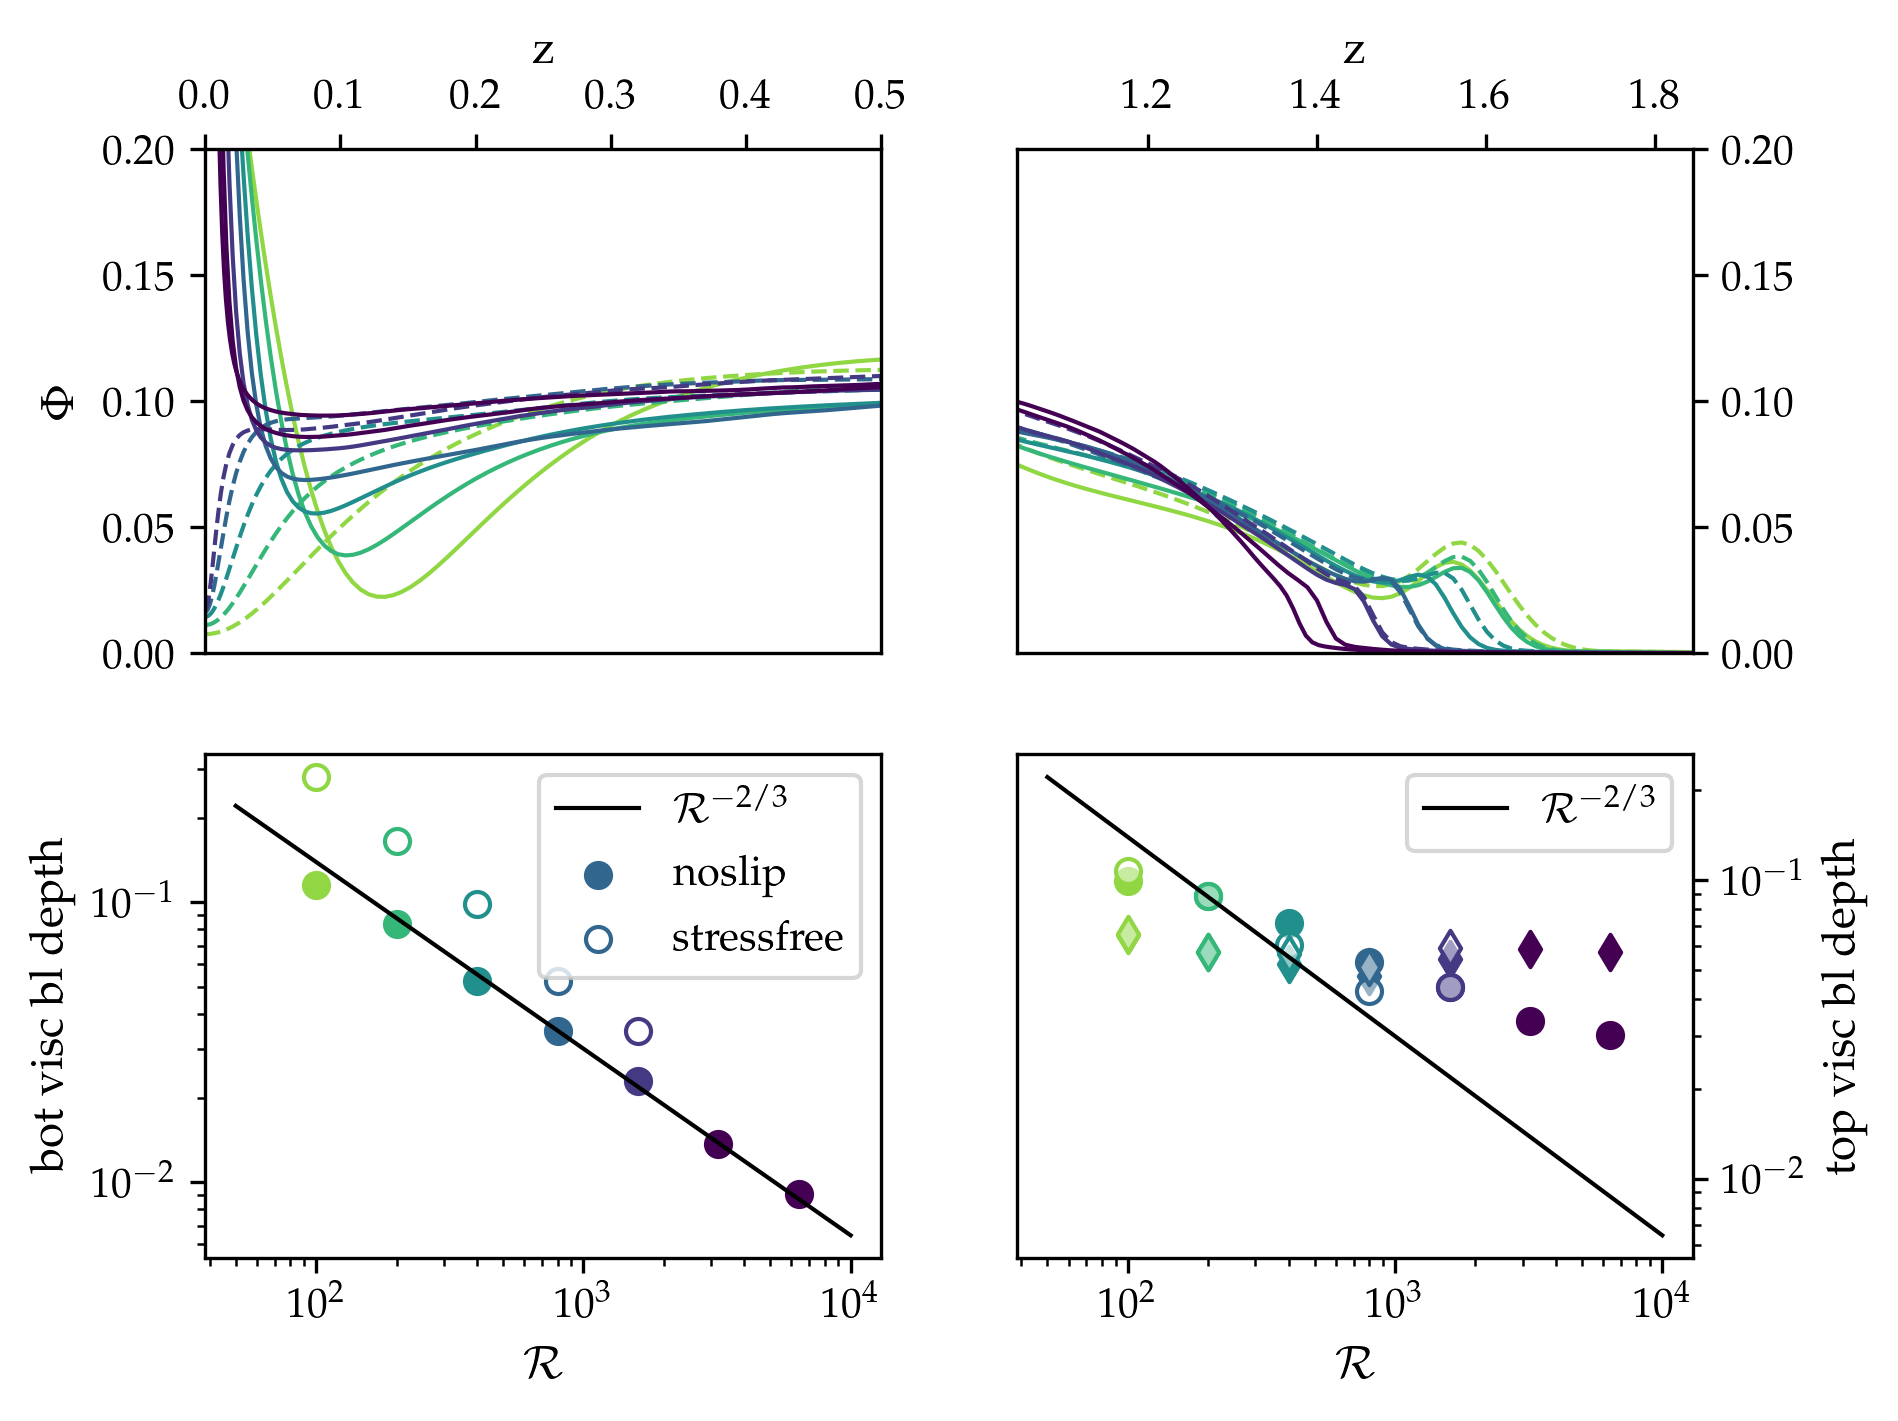
\includegraphics[width=0.95\textwidth]{viscous_boundary_layers.png}
\caption{
(Upper left) Dissipation profiles \emph{near the bottom boundary} for no-slip (solid lines) and stress-free (dashed lines) at various $\mathcal{R}$ (more purple = higher $\mathcal{R}$).
(Upper right) Dissipation profiles in the PZ.
We see large differences in morphology near the bottom boundary for different boundary condition choices, but not in the PZ.
(Bottom left) Viscous boundary layer length scales vs.~$\mathcal{R}$ with the prediction from standard RBC overplotted.
The fit is good.
(Bottom right) Viscous boundary layer length scales (circles) and penetration zone widths ($\delta_{0.9} - \delta_{0.1}$, diamonds) are compared.
At low $\mathcal{R}$, perhaps the classical RBC BL scaling applies.
Once the viscous BL becomes smaller than the width of the ``thermal adjustment layer'' (the thermal boundary layer, a constant for all of these simulations), the scaling levels out.
The viscous boundary layer also becoems much less pronounced in the PZ for these high-$\mathcal{R}$ simulations (see e.g., upper right).
\label{fig:profiles}
}
\end{figure}

\begin{figure}[ht!]
\centering
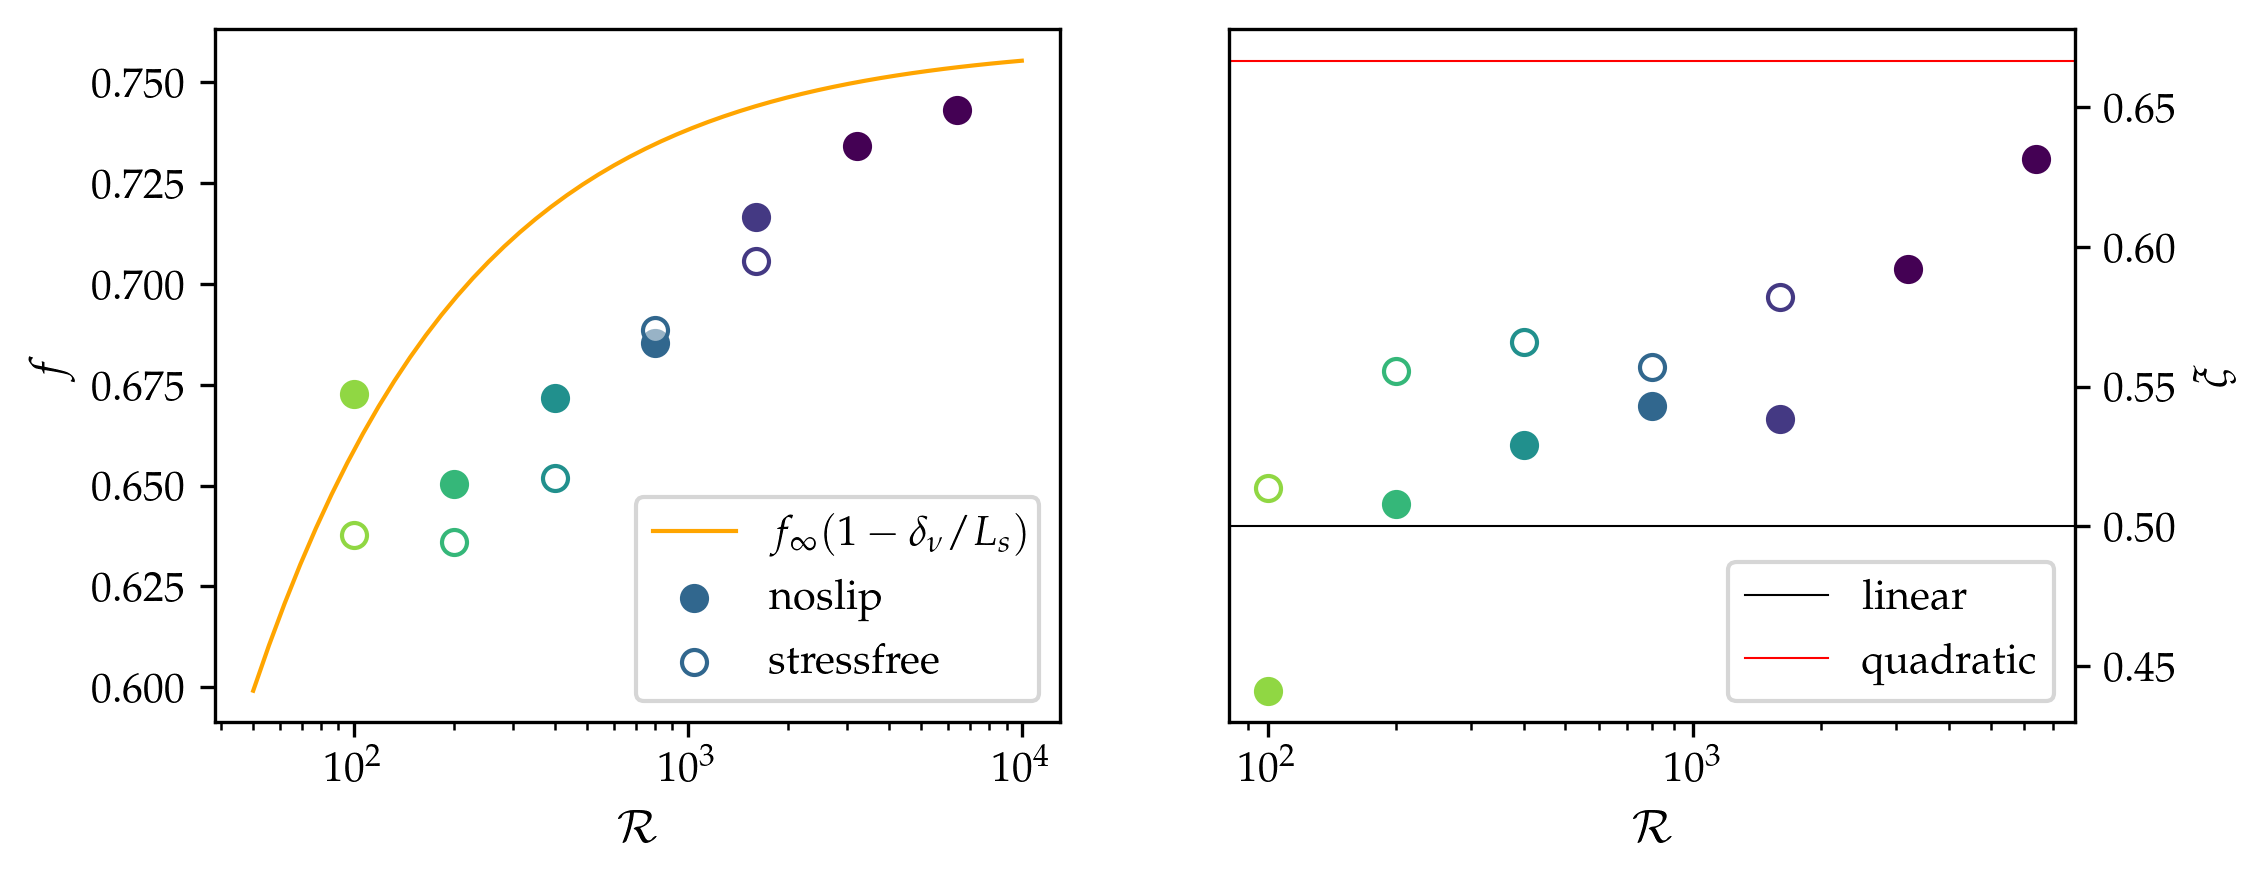
\includegraphics[width=\textwidth]{f_scaling.png}
\caption{
(Left) measured values of $f$ from the data over the full CZ from $z = [0, L_s]$.
The simple prediction of Eqn.~\ref{eqn:stressfree_f} is overplotted with $f_{\infty} = 0.76$.
(Right) geometric factor $\xi$ calculated by rearranging Eqn.~\ref{eqn:xi_defn}.
We see that a linear description of PZ dissipation is decent at low $\mathcal{R}$ but at higher $\mathcal{R}$ a quadratic description is better.
A logical upper bound for $\xi$ is 1, and that could be used to provide a lower limit for the size of PZs in the infinite-$\mathcal{R}$ limit.
\label{fig:f_and_xi}
}
\end{figure}


\bibliography{biblio.bib}
\end{document} 
